\chapter{Tie Strength} % (fold)
\label{cha:tie_strength}
    \section{Critical threshold} % (fold)
    \label{sec:critical_threshold}
        As described in chapter 8 of \cite{network_science}, we have obtained the \textbf{critical threshold}
        representing the fraction of the nodes that have to be removed to break apart out network. This fraction,
        represented by $f_c$, is obtained by the following formula:

        \begin{equation*}
            f_c = 1 - \frac{1}
            {\frac{\gamma - 2}{3 - \gamma}k^{\gamma - 2}_{\mathit{min}}k^{3 - \gamma}_{\mathit{max}} \ - \  1} =
            1 - \frac{1}{1.50 * 1^{0.6} * 19073^{0.4} \ - \ 1} = 0.99
        \end{equation*}

        which, remembering that the $\gamma$ for our scale-free network corresponds to $2.6$ and that
        $k_{\mathit{min}}$ and $k_{\mathit{max}}$ are eguals to $1$ and $19073$ respectively, tells us that, in
        order to break apart our network it is mandatory to remove the $99\%$ of the nodes. Keeping in mind that
        our network is, in fact, a finite network, we can adjust the obtained result by utilizing the following
        formula, still described in chapter 8 of \cite{network_science}:

        \begin{equation*}
            f_c \approx 1 - \frac{C}{N^{\frac{3 - \gamma}{\gamma - 1}}} \approx 1.00
        \end{equation*}

        where $C = \frac{1}{\sum_{k=1}^{\infty}k^{-\gamma}}$ is a constant and $N$ represents the number of nodes
        of the network. As we can see, this new approximation tells us that in order to break apart our network the
        totality of its nodes has to be removed.
    % section critical_threshold (end)
    \section{Simulation of an attack} % (fold)
    \label{sec:simulation_of_an_attack}
        In order to validate the results obtained in Section \ref{sec:critical_threshold}, here we simulate an
        attack to our network. We've chosen to simulate the remotion of $50$ nodes from the network following two
        distinct criterions: \textbf{random selection} and \textbf{degree centraility} (decreasing order). For every
        criterion we've monitored the spreading of the connected components

        \begin{figure}[H]
            \centering
            \begin{subfigure}{0.45\textwidth}
                \resizebox{\textwidth}{!}{
                    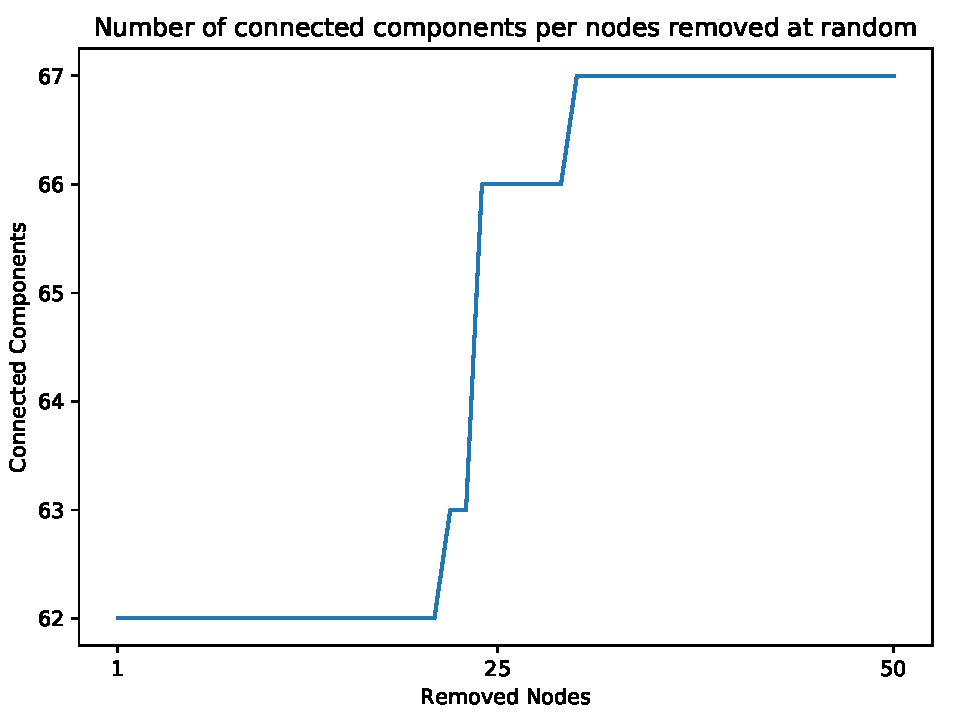
\includegraphics{images/tie_strength/test_cc_on_random.pdf}
                }
                \caption{}
                \label{test_cc_on_random}
            \end{subfigure}
            \begin{subfigure}{0.45\textwidth}
                \resizebox{\textwidth}{!}{
                    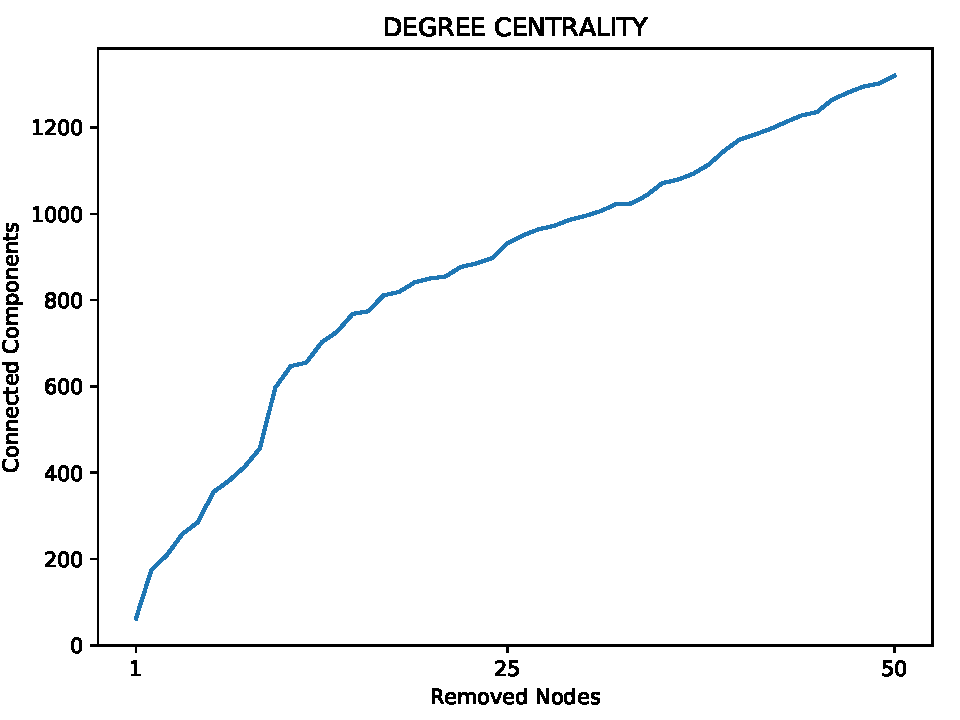
\includegraphics{images/tie_strength/test_cc_on_degree_centrality.pdf}
                }
                \caption{}
                \label{test_cc_on_degree_centrality}
            \end{subfigure}
            \caption{}
            \label{test_cc}
        \end{figure}
    % section simulation_of_an_attack (end)
% chapter tie_strength (end)
